%Latex2e file
\documentclass[12pt,letterpaper]{article}
%\renewcommand{\arraystretch}{2}
%\input{\scrload.tex}
\setlength{\textwidth}{6.5in}
\setlength{\textheight}{8.6in}

\setlength{\oddsidemargin}{-.25in}
\setlength{\evensidemargin}{-.25in}
\setlength{\topmargin}{-.25in}
\pagestyle{empty}

\usepackage{amsmath}
\usepackage{amssymb}
\usepackage{graphicx}

\newcommand{\R}{\ensuremath{{\mathbb{R}}}}
\newcommand{\Z}{\ensuremath{{\mathbb{Z}}}}
\newcommand{\Q}{\ensuremath{{\mathbb{Q}}}}
\newcommand{\N}{\ensuremath{{\mathbb{N}}}}
\newcommand{\C}{\ensuremath{{\mathbb{C}}}}
\newcommand{\Proof}{\noindent {\bf Proof: }}
\newcommand{\QED}{\begin{flushright}QED\end{flushright}}
\newcommand{\Refl}{{\bf Reflexive: }}
\newcommand{\Symm}{{\bf Symmetric: }}
\newcommand{\Tran}{{\bf Transitive: }}
\newcommand{\ep}{\varepsilon}
\newcommand{\ri}{\right|}
\newcommand{\lef}{\left|}
\newcommand{\toR}{\to \R}
\newcommand{\fancy}[1]{#1_{\text{fancy}}}
\newcommand{\pro}[1]{\noindent {\bf #1}}
\newcommand{\prob}[1]{\newpage\noindent {\bf #1}}
\newcommand{\bacon}{\approx}

   
\begin{document}
\begin{flushright}
Nick Kerner

Homework 8

Chapter 6: 9

Dr Frey's Bonus but required fun question

Chapter 7: K2, K3, K5

\end{flushright}
\begin{center}
\large{Geometry}\\
\end{center}

\pro{Chapter 6: problem 9 } Assume that parallel lines $l$ and $l'$ have a common perpendicular $\overleftrightarrow{PQ}$.  For any point $X$ on l, let $X'$ be the foot of the perpendicular from X to $l'$. Prove that as X recedes endlessly from P on l, the segment XX' increases indefinitely;  \\





Given $X\neq P $ on l, by proposition 6.6 we know there are two limiting parallel rays to $l'$ emanating from P (on opposite sides of $\overleftrightarrow{PQ}$.  Choose the one on the same side of $\overleftrightarrow{PQ}$ as X and drop a perpendicular from X to our limiting parallel ray and call the foot Y.   Know we know that $\overrightarrow{PY}$ is interior to $\angle QPX$ ($\overrightarrow{PY}\neq \overrightarrow{PX}$ as limiting parallel rays cannot have a common perpendicular to their respective line by Hilbert's Hyperbolic axiom of parallels, so XY is a segment not a point). \\

Case 1: $\overrightarrow{PY}$ is interior to $\angle XPX'$\\

Then by crossbar theorem we know that $\overrightarrow{PY}$ must intersect $XX'$. \\

Case 2: $\overrightarrow{PY} = \overrightarrow{PX'}$\\

Our limiting parallel cannot intersect $l'$.  Contradiction.\\

Case 3: $\overrightarrow{PY}$ is interior to $\angle QPX'$.\\

By crossbar theorem, $\overrightarrow{PY}$ intersects $QX'$, but our limiting parallel cannot intersect $l'$.  Contradiction.\\

Therefore we know that $\overrightarrow{PY}$ intersects $XX'$ (not at an endpoint as it would be the parallel with common perpendicular to $l'$ or it would intersect $l'$) call this point Z.  \\

Case 1: Y = Z.\\

$XY = XZ$, clearly. \\

Case 2: $Y\neq Z$.\\

Consider $\triangle XYZ$.  We know that $\angle XYZ$ is a right angle, so its measure is $90^\circ$, so since we are in hyperbolic a triangle's angle sum must be less than 180, so both other angles have measures less than $90^\circ$.  So we know by proposition 4.5 that since $\angle XYZ > \angle XZY$ then $XZ > XY$.\\

Hence $XZ \geq XY$.\\

To use Aristotle's axiom, we must show that $\angle XPY$ is acute. Now we know that $\angle QPY$ is acute (proposition 6.6) and we know that it is interior to $\angle QPX$ which is right, so by angle subtraction we know that $\angle XPY$ is acute. \\

By Aristotle's axiom, given any segment AB (A on l, B on $\overrightarrow{PY}$), there is some X with foot Y such that $XY > AB$.  So we know by segment addition that $XX' > XZ \geq XY > AB$. 

\QED 









\prob{Dr Frey's Bonus but required fun question }

Let $\triangle ABC$ be any traingle, and let L,M, and N  be the midpoints of BC, AB, and AC, respectively. Prove that $\triangle AMN$ is not similar to $\triangle ABC$.  Prove that MN is not congruent to BL by assuming the contrary and deducing that $\triangle ABC$ has angle sum $180^\circ$. Show that $\triangle ANM \cong \triangle CND$, then that $\triangle MDC \cong \triangle CBM$. Substitute appropriately in the equation $180^\circ = \angle BMC^\circ + \angle CMD ^\circ + \angle AMN ^\circ$.\\

%AMN is not similar to ABC



\Proof

Assume to the contrary that $\delta (AMN) = \delta (ABC)$. By proposition 6.1 we know that $\delta (ABC) = \delta(MCB) + \delta (MCA)$.  Additionally we know that $\delta (MCA) = \delta (MNC) + \delta (AMN)$, so we know that $\delta (ABC) = \delta(MCB) + \delta (MCA) = \delta(MCB) + (\delta (MNC) + \delta (AMN)) = \delta(MCB) + \delta (MNC) + \delta (ABC)$.  Therefore $\delta (MCB) + \delta (MNC) = 0$ so $\delta (MCB)= 0$ and $\delta (MNC) = 0$.  Contradiction.  Hence $\triangle AMN$ and $\triangle ABC$ cannot be similar. 

\QED


%MN \not \cong BL
\Proof

Assume to the contrary that $MN \cong BL$.  Choose D such that $M*N*D$ and $ND \cong MN$. So $\angle CND$ and $\angle MNA$ are vertical angles, $MN\cong ND$ and $AN \cong NC$ so by SAS we know that $\triangle ANM \cong \triangle CND$.\\

So we know that $BM \cong MA \cong DC$.\\


Additionally we know that 

\begin{eqnarray*}
MD &=& MN + ND \\
&\cong & MN + MN \\
&\cong & BL + BL \\
&\cong & BL + LC\\
&=& BC
\end{eqnarray*}

and $MC \cong MC$ so by SSS we know that $\triangle MBC \cong \triangle CDM$.\\


Finally we know that $\angle BMC^\circ + \angle CMD^\circ + \angle DMA^\circ = 180$ as they make a straight line.  So (substitutions are either renaming angles or derived from congruent triangles).\\

\begin{eqnarray*}
180 &=& \angle BMC^\circ + \angle CMD^\circ + \angle DMA^\circ\\
&=& \angle MCD^\circ + \angle CMD^\circ + \angle DMA^\circ\\
&=& (\angle MCN^\circ + \angle NCD^\circ) + \angle CMD^\circ + \angle DMA^\circ\\
&=& \angle MCN^\circ + \angle NAM^\circ + \angle CMD^\circ + \angle DMA^\circ\\
&=& \angle NAM^\circ + \angle MCN^\circ + \angle CMD^\circ + \angle DMA^\circ\\
&=& \angle NAM^\circ + \angle MCN^\circ + \angle MCB^\circ + \angle DMA^\circ\\
&=& \angle NAM^\circ + (\angle MCN^\circ + \angle MCB^\circ) + \angle DMA^\circ\\
&=& \angle NAM^\circ + \angle NCB^\circ + \angle DMA^\circ\\
&=& \angle CAB^\circ + \angle ACB^\circ + \angle DMA^\circ\\
&=& \angle CAB^\circ + \angle ACB^\circ + \angle MDC^\circ\\
&=& \angle CAB^\circ + \angle ACB^\circ + \angle CBM^\circ\\
&=& \angle CAB^\circ + \angle ACB^\circ + \angle CBA^\circ
\end{eqnarray*}

So $\delta (ABC) = 0$.  Contradiction.


\QED







\prob{Chapter 7: K2 }

a. Let $l$ be a diameter of $\gamma$ and let $m$ be an open chord of $\gamma$ that does not meet $l$ and whose endpoints differ from the endpoints of $l$. Draw a diagram showing the common perpendicular $k$ to $l$ and $m$ in the Klein model.

\begin{center}
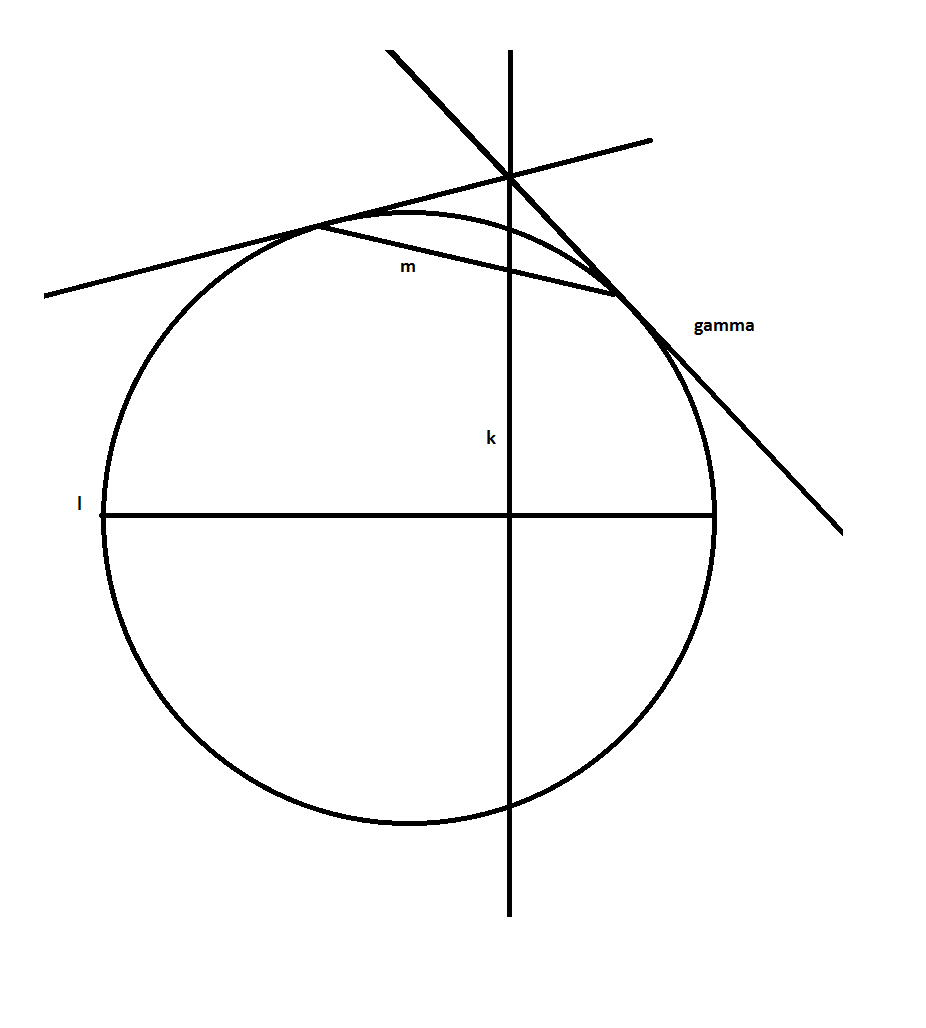
\includegraphics[width=2in]{klein2.png}
\end{center}


b. Let $l$ and $m$ be intersecting open chords of $\gamma$. It is a valid theorem in hyperbolic geometry that for any two intersecting nonperpendicular lines there exists a third line perpendicular to one of them and asymptotically parallel to the other (see ME 9, Ch. 6). Draw the two lines in the Klein model that are perpendicular to $l$ and asymptotically parallel to $m$ (on the left and right, respectively). This shows that the angle of parallelism can be any acute angle whatever. Explain. \\


\begin{center}
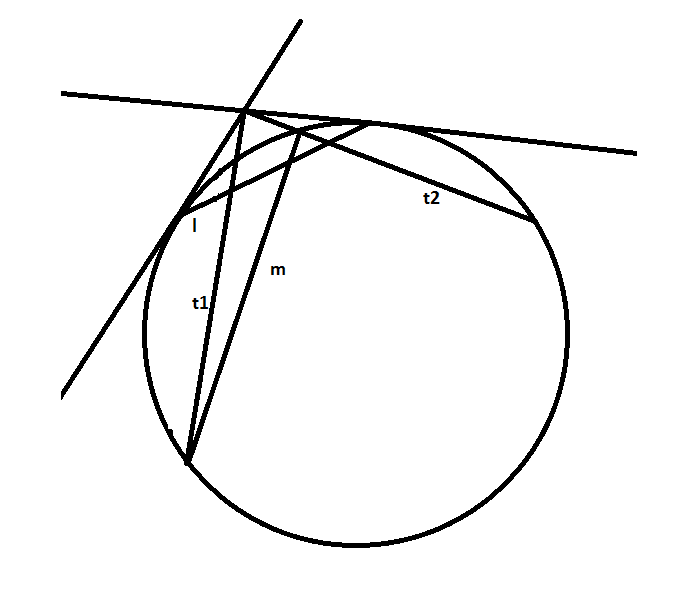
\includegraphics[width=2in]{klein2b.png}
\end{center}

Note that two lines, m and l, can intersect at whatever angle they want.  As long as m is not perpendicular to l, then we can create a transversal perpendicular to l that is asymptotically parallel to m.  So our angle of parallelism can be whatever acute angle m and l intersect at (for the obtuse angles, they are supplementary to an acute angle and the acute angle has the ray that will be asymptotically parallel to our transversal as otherwise our triangles would have more than 180 degrees to their angle sum).\\


\newpage 
c. In the Euclidean plane, any three parallel lines have a common transversal. Draw three parallel lines in the Klein model that do \emph{not} have a common transversal.\\

\begin{center}
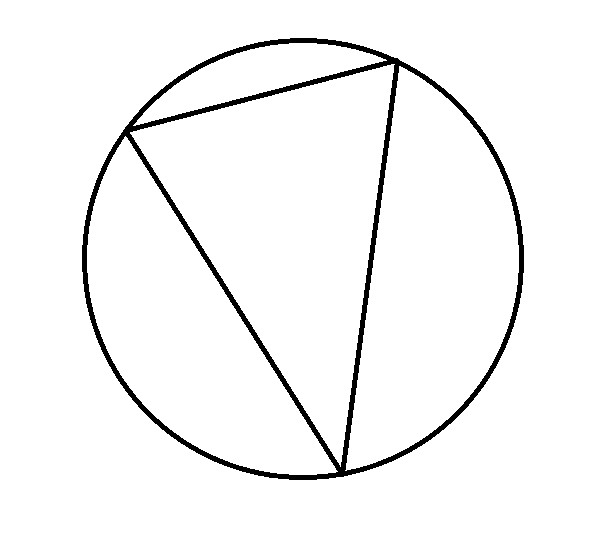
\includegraphics[width=2in]{Threepar.png}
\end{center}


\prob{Chapter 7: K3 }

a. In the Klein model, an ideal point and an ordinary point always determine a unique Klein line. Translate this back into a theorem in hyperbolic geometry about limiting parallel rays.\\

An ideal point and an ordinary point make a unique Klein line.  However, we know that each line is associated with 2 ideal points.  Given any ordinary point not on our line, we can create two asymptotically parallel rays to our line (limiting parallel rays).  In the Euclidean plane, these are segments which contain our point and our ideal point.  Additionally, if we drop a foot from our point to our line, both rays will be on opposite sides of that line (as the ideal points must be on opposite sides of the line).  This is effectively proposition 6.6.\\

Additionally, we can see that limiting parallelism is symmetric almost trivially, as two rays are limiting parallel to each other if they share and ideal endpoint.  Also we can get transitivity, if m and l are limiting parallel rays to each other, and l and k are limiting parallel rays to each other (and the rays going the same direction, ie we are using l to mean the same ray, not just rays on the same line, in both statements) then k share the same endpoint that m and l share, so k is limiting parallel to m as well because they share an endpoint. \\

Another theorem you could make up is to say that if you have a point and a direction, you can determine a unique line in hyperbolic geometry. \\


\newpage 
b. Suppose the ultra-ideal points P($l$) and P($m$) are poles of Klein lines $l$ and $m$, respectively. You saw in Figure 7.18 that the Euclidean line joining P($l$) and P($m$) need not cut through the circle $\gamma$ and hence need not determine a Klein line. Show that the only case in which there is a Klein line joining P($l$) and P($m$) is when lines $l$ and $m$ are divergently parallel. \\


Note, to have poles our lines cannot be diameters.\\

Case 1: Lines are limiting parallel (asymptotically parallel), they ``meet'' at an ideal point.\\

The pole is found by using the tangent lines of the ideal ends of each Klein line.  However, one of these points is shared, so two points along the same tangent line are the poles of our two lines.  However, we know two points make a unique line, so this line is tangent to the circle, and therefore does not create a Klein line as tangent lines do not enter the circles they are tangent to. \\

Note above, if the poles are the same point, then we get both same ideals, which means that $m=l$.\\


Case 2: Lines intersect\\

Consider two lines l and m which intersect.  So we know the ideal points of one line are on opposite sides of the other Klein line.  Let the tangent lines of l be $l_1$ and $l_2$ and let their respective ideal points be $L_1$ and $L_2$.  Similarly let the tangent lines of m be $m_1$ and $m_2$ and let their respective ideal points be $M_1$ and $M_2$. \\


So we know that every point in the Klein model lies on one side of a tangent ``line'', as the entire circle must.  Consider $P(l)$, so we know that every point contained in the circle is interior to $\angle l_1 P(l) l_2$ as each ordinary point and ideal point are on the same side of a tangent line except for the point of tangency.  So every point in $\gamma$ is on the same side of $l_1$ as $L_2$ and on the same side of $l_2$ as $L_1$. Additionally, we know that either $M_1$ or $M_2$ is on the same side of l as $P(l)$, without loss of generality let it be $M_1$.  So we know that $M_1$ is interior to every angle of $\triangle L_1L_2P(l)$, so it is interior to the triangle.  So consider half of the tangent line at $P_1$.  This is a ray emanating from the interior of our triangle, so it must intersect a side or vertex of the triangle. Note, it cannot intersect $L_1$ or $L_2$ as that would mean that m would be asymptotically parallel to l (case 1), also it cannot intersect P(l) as there are only two tangent lines that do this, they are $l_1$ and $l_2$.  Therefore if this ray intersects $P(l)$ then m and l share an ideal point, so they are either asymptotically parallel (so they cannot intersect) or they are the same line.  Contradiction.  Therefore the line tangent at $M_1$ cannot intersect a vertex of $\triangle L_1L_2P(l)$.\\

Therefore, since a tangent ray emanating from $M_1$ cannot intersect a vertex of $\triangle L_1L_2P(l)$.   We know that the tangent line must therefore intersect two sides (first take a tangent ray, it leaves the triangle through a side, pick a point on this ray and take another ray pointing back into the triangle and use Pasch's theorem).  However, if we suppose it intersects $L_1L_2$ then it must enter the circle (and therefore exit it through another point) so it is not a tangent line. \\

Therefore $m_1$ must intersect both $L_1P(l)$ and $L_2P(l)$ not at an endpoint, so $K_1 * M_1 * K_2$ where $K_1$ is where $m_1$ intersects $l_1$ and $K_2$ is where $m_1$ intersects $l_2$.\\

Similarly, since $L_1$ and $L_2$ are on opposite sides of m, we know that either $l_1$ or $l_2$ (WLOG $l_2$) must intersect both $M_1P(m)$ and $M_2P(m)$ not at endpoints, so $J_1 * L_2 * J_2$ where $J_1$ is where $l_2$ intersects $m_1$ and $J_2$ is where $l_2$ intersects $m_2$.\\

Therefore we know that $J_1 = K_2$ as they are both the intersection of lines we know to be distinct.  Therefore we know that $K_1 * M_1 * K_2 * P(m)$ as $K_2 = J_1$ is where $l_2$ intersects $m_1$ between $M_1$ and $P(m)$, so we know that $M_1$ and $P(m)$ are on the same side of $l_1$ ($l_1$ contains $K_1$ and does not contain $M_1, K_2,$ or $P(m)$ as that would mean $l_1 = m_1$).  Also, as we stated earlier, all ideal points and ordinary points except the point of tangency will be on the same side of a tangent line, so the ordinary points of $\gamma$ and $P(m)$ are on the same side of $l_1$.\\

Also, since $M_1 * K_2 * P(m)$ we know that $M_1$ and $P(m)$ are on opposite sides of $l_2$ ($K_2 \in l_2$ and the other two points are not).  Therefore since $M_1$ and the ordinary points of $\gamma$ will be on the same side of $l_2$, the ordinary points of $\gamma$ are on the side of $l_2$ opposite P(m).\\

Therefore consider the rays $\overrightarrow{P(l)X}$ and $\overrightarrow{P(l)P(m)}$ where $X*P(l)*P(m)$.  Note that, except for $P(l) \not\in\gamma$, $\overrightarrow{P(l)X}$ is on the opposite side of $l_1$ from $P(m)$, so $\overrightarrow{P(l)X}$ is on the opposite side of $l_1$ from the ordinary points of $\gamma$.  Similarly we know that, except for $P(l) \not\in\gamma$, $\overrightarrow{P(l)P(m)}$ is on the opposite side of $l_2$ from the ordinary points of $\gamma$.  Therefore $\overleftrightarrow{P(m)P(l)}$ does not intersect $\gamma$.\\




Case 3: Lines are divergently parallel\\

By theorem 6.3 we know there is a common perpendicular between these two lines.  To be perpendicular to these lines, it must go through the poles of the lines (these lines cannot be diameters).  Therefore the poles do determine a Klein line in this case.

\QED


\newpage

c.  Suppose the ultra-ideal point P($l$) is the pole of a Klein line $l$ and $\Omega$ is an ideal point; $\Omega$ is uniquely determined by a ray $r$ in the direction of $\Omega$. State the necessary and sufficient conditions on $r$ and $l$ in order that P($l$) and $\Omega$ determine a Klein line. Translate this into a theorem in hyperbolic geometry. \\

Necessary and sufficient conditions on r and l in order that P(l) and $\omega$ determine a Klein line: \\

The ray r cannot be limiting parallel to l (l cannot be a diameter if it has a pole).  Then $\omega$ will be an ideal point interior to the angle created by the endpoints of l and P(l).  By the crossbar theorem, $\omega$ and $P(l)$ determine a line that intersects l, so we know it intersects the circle twice and therefore is a Klein line.\\

Result in Hyperbolic: \\

Given a line l and a ray r that is not limiting parallel to l, there is a unique line perpendicular to l that r is limiting parallel to.  



\prob{Chapter 7: K5 } Use the Klein model to show that in the hyperbolic plane there exists a pentagon with five right angles and there exists a hexagon with six right angles. (See hint.) Does there exist for all $n\geq 5$ an $n$-sided polygon with $n$ right angles?\\

\noindent Pentagon:\\


Let l and m be two divergently parallel lines where the end points of l and m are $L_1$, $L_2$, $M_1$, and $M_2$ such that $M_1$ and $L_1$ are on the same side of q and l and m are on opposite sides of a diameter perpendicular to q. 


So take some ray r interior to $\angle M_1P(l)L_1$. Assume to the contrary that this ray intersects m, call this point of intersection X.  So we know that $M_1*X*M_2$ and we know that $X$ and $L_1$ are on the same side of $\overrightarrow{P(l)M_1}$. Additionally, all ideal and ordinary points except $L_1$ are on the same side of $\overrightarrow{P(l)L_1}$. Therefore $X$ and $M_2$ are both interior the $\angle M_1P(l)L_1$. Therefore q must also be interior to $\angle M_1 P(l)L_1$ so it can cut $M_1L_2$.  Therefore it cuts $M_1L_1$. Contradiction.  Therefore it does not intersect m.\\

Additionally, since $M_1$ is an ideal point other than $L_1$ or $L_2$ then $\overrightarrow{P(l)M_1}$ must intersect l.  Therefore by the crossbar theorem, r must intersect l. Since r goes through $P(l)$ and intersects l, it is perpendicular to l. \\

Next, since r enters $\gamma$, it must also exit $\gamma$.  So r contains a Klein line, call it w.\\



Finally, connecting the poles of w and m will create 2 more right angles, for a total of 5 right angles, additionally we have a total of 5 sides.  So we have a pentagon with 5 right angles. \\ 
  

\noindent Hexagon:\\

With exception to the last step provided in the pentagon proof, do everything the same.  Then, repeat the same process finding a ray interior to $\angle A_1P(a)M_1$ where $A_1$ is the ideal point of $a$ ``closer'' to $P_1$.  That is, the ideal point of a on the same side of $\overleftrightarrow{OP(a)}$ as $M_1$ (originally we divided $\gamma$ into four quarters, one with $L_1$, one with $M_1$ etc.  We chose $A_1$ in such a way as to force it to be in the quarter with $L_1$ or $M_1$, so its diametric opposite must be in one of the other two quarters (the two possible quarters are adjacent, not diagonal)).\\

Next, recognize that that ray can determine a Klein line, call it h, and connect $P(h)$ to $P(a)$ and connect $P(h)$ to $P(m)$.  Notice since we have connected poles, all angles made are perpendiculars and we have 6 of them in our closed hexagon. 







\newpage

\noindent Does there exist, for all $n \geq 5$, an n-sided polygon with n right angles?  \\

Yes.  Note the process for the pentagon.  We start with two parallel lines with a mutual perpendicular.  Then we follow the following steps to increase the number of sides of our incomplete polygon, making sure never to allow the ideal points on each end to coincide.\\

If we wish to increase the number of sides the incomplete shape has by 1, then we draw a new line from the pole of one of our ends such that it does not intersect any of our other sides (except the side it is a pole of) and make sure our expansion is on the appropriate side of our original mutual perpendicular, namely the same side that all previous expansions, if there have been any, have been on.  Then we take the new line and find its pole.  Now we have 1 additional side to our polygon and we note that it is perpendicular to what was previously the end-side of our incomplete polygon.  Note that starting from two parallel lines with a mutual perpendicular we can create an incomplete shape with any number of sides $n \geq 4$.  Then, when we have 1 less than the number of sides we must create, we connect our pole from one end to the pole of the other end of our construction, which causes our new line to be a mutual perpendicular to both ends of our polygon which is now complete.

\end{document}